\documentclass[14pt,aspectratio=169,compress]{beamer}
\usetheme{Copenhagen}
% something tries to renewcommand these but beamer must break the assumption that they are defined so I am defining them
\newcommand{\labelitemi}{}
\newcommand{\labelitemii}{}
\newcommand{\labelitemiii}{}
\newcommand{\labelitemiv}{}

\usepackage{greg}

\useoutertheme[subsection=false]{miniframes}
\useinnertheme{circles}
\setbeamertemplate{navigation symbols}{}
\setbeamercovered{transparent}
\definecolor{cmu_red}{RGB}{153,0,0} % #990000
\definecolor{cmu_dark_red}{RGB}{100,0,0} % #990000
\definecolor{classical}{RGB}{240, 250, 240} % #464646
\definecolor{cmu_dark_grey}{RGB}{70, 70, 70} % #464646
\usecolortheme[named=cmu_red]{structure}
\setbeamercolor{palette secondary}{bg=cmu_dark_grey,fg=white}
\setbeamercolor{palette tertiary}{bg=cmu_dark_red,fg=white}
\setbeamercolor{section in head/foot}{bg=cmu_red,fg=white}

% \setbeamercolor{corollary title}{use=structure,fg=white,bg=structure.fg!75!black}
% \setbeamercolor{corollary body}{parent=normal text,use=block title,bg=blue}
%\setlength{\parskip}{\baselineskip} 

\title[Geometry in HoTT]{DRAFT: Discrete differential geometry in homotopy type theory}
\author{Greg Langmead}
\institute[CMU]{Carnegie Mellon University}
\logo{
\includegraphics[width=100pt]{figs/cmu-wordmark-horizontal-r.pdf}}
\date{April 2025}

\begin{document}
\begin{frame}
\titlepage
\end{frame}

\begin{frame}
\tableofcontents
\end{frame}

\section{Introduction}

\begin{frame}{Motivation}
The motivation is to provide \alert{a deeper explanation} for \alert{Chern-Weil theory} by finding \alert{connections} and \alert{curvature} in HoTT \alert{principal bundles}.
\end{frame}

% {
% \setbeamercolor{background canvas}{bg=classical}
% }

\section{The plan}
\begin{frame}
\begin{itemize}
\item Construct a classifying space of principal bundles
\item Construct a type of manifolds
\item Identify connections and curvature
\item Put these to use in 2-d to prove that total curvature is an integer
\end{itemize}
\end{frame}

\section{Classifying space}

\begin{frame}
\begin{definition}
Let \( G \) be a group with identity element \( e \). A \defemph{\( G \)-set} is a set \( X \) equipped with a homomorphism \( \phi:(G,e)\to\Aut(X) \). If we have
\[ 
\mathsf{is\underscore torsor}(X,\phi)\defeq ||X||_{-1}\times \pit{x:X}\mathsf{is\underscore equiv}(\phi(-,x):(G,e)\to (X,x))
\] we say \( (X,\phi) \) is a \defemph{\( G \)-torsor}. Denote the type of \( G \)-torsors by \( BG \).
\end{definition}
\begin{lemma}
Point \( BG \) at \( \reg{G} \), the \( G \)-torsor \( G \) acting on itself on the right. Then \( \loopy_{\reg{G}} BG \simeq G \), so \( BG \) is a \( \K(G,1) \).
\end{lemma}
\end{frame}

\begin{frame}
\begin{definition}
\( \EM(G,n)\defeq \BAut(\K(G,n))\defeq \sit{Y:\uni}||Y\simeq \K(G,n)||_{-1} \)
\end{definition}
\begin{definition}
A \defemph{\( \K(G,n) \)-bundle} on a type \( M \) is a map \( f:M\to \EM(G,n) \).
\end{definition}
We further assume \( f \) factors through \( \K(G,n+1) \) and so is principal.
\end{frame}

\section{Discrete manifolds}

\begin{frame}{Discrete manifolds in HoTT}
\begin{itemize}
\item Recall the classical theory of \alert{simplicial complexes}
\item Define a \alert{realization} functor via higher inductive types (pushouts)
\end{itemize}
\end{frame}

\begin{frame}{Simplicial complexes}
\begin{columns}
\begin{column}{0.5\textwidth}
\!\!\!\!\!\vspace{-0.5cm}\resizebox{220pt}{!}{
\begin{tikzpicture}[scale=0.1]
    \matrix (A) [matrix of math nodes, row sep=1cm, column sep=-.2cm]
    { 
       ~ &  ~ & ~ & ~ & ~ & \left\{\substack{{w, b, r}\\ {g, o, y}}\right\} \\  
  ~ &  ~ & \scriptstyle\{w, b, r\} & \scriptstyle\{w, r, g\}  & \scriptstyle\{w, g, o\} & \scriptstyle\{w, o, b\} & \scriptstyle\{y, b, r\} & \scriptstyle\{y, r, g\}  & \scriptstyle\{y, g, o\} & \scriptstyle\{y, o, b\}\\
  \scriptstyle\{w, b\} & \scriptstyle\{w,r\}  & \scriptstyle\{w,g\} & \scriptstyle\{w,o\} & \scriptstyle\{b, r\} & \scriptstyle\{r, g\}  & \scriptstyle\{g, o\} & \scriptstyle\{o, b\} & \scriptstyle\{y, b\} & \scriptstyle\{y,r\}  & \scriptstyle\{y,g\} & \scriptstyle\{y,o\}\\
  ~ & ~ & ~ &  \scriptstyle\{w\}  & \scriptstyle\{b\} & \scriptstyle\{r\} & \scriptstyle\{g\} & \scriptstyle\{o\} & \scriptstyle\{y\}\\
      ~ & ~ &  ~ & ~ & ~ & \emptyset \\
    };
    \draw (A-1-6.south)--(A-2-3.north);
    \draw (A-1-6.south)--(A-2-4.north);
    \draw (A-1-6.south)--(A-2-5.north);
    \draw (A-1-6.south)--(A-2-6.north);
    \draw (A-1-6.south)--(A-2-7.north);
    \draw (A-1-6.south)--(A-2-8.north);
    \draw (A-1-6.south)--(A-2-9.north);
    \draw (A-1-6.south)--(A-2-10.north);

    \draw (A-2-3.south)--(A-3-1.north);
    \draw (A-2-3.south)--(A-3-2.north);
    \draw (A-2-3.south)--(A-3-5.north);

    \draw (A-2-4.south)--(A-3-2.north);
    \draw (A-2-4.south)--(A-3-3.north);
    \draw (A-2-4.south)--(A-3-6.north);

    \draw (A-2-5.south)--(A-3-3.north);
    \draw (A-2-5.south)--(A-3-4.north);
    \draw (A-2-5.south)--(A-3-7.north);

    \draw (A-2-6.south)--(A-3-4.north);
    \draw (A-2-6.south)--(A-3-1.north);
    \draw (A-2-6.south)--(A-3-8.north);

    \draw (A-2-7.south)--(A-3-5.north);
    \draw (A-2-7.south)--(A-3-10.north);
    \draw (A-2-7.south)--(A-3-9.north);

    \draw (A-2-8.south)--(A-3-6.north);
    \draw (A-2-8.south)--(A-3-11.north);
    \draw (A-2-8.south)--(A-3-10.north);

    \draw (A-2-9.south)--(A-3-7.north);
    \draw (A-2-9.south)--(A-3-12.north);
    \draw (A-2-9.south)--(A-3-11.north);

    \draw (A-2-10.south)--(A-3-8.north);
    \draw (A-2-10.south)--(A-3-9.north);
    \draw (A-2-10.south)--(A-3-12.north);

    \draw (A-3-1.south)--(A-4-4.north);
    \draw (A-3-1.south)--(A-4-5.north);

    \draw (A-3-2.south)--(A-4-4.north);
    \draw (A-3-2.south)--(A-4-6.north);

    \draw (A-3-3.south)--(A-4-4.north);
    \draw (A-3-3.south)--(A-4-7.north);

    \draw (A-3-4.south)--(A-4-4.north);
    \draw (A-3-4.south)--(A-4-8.north);

    \draw (A-3-5.south)--(A-4-5.north);
    \draw (A-3-5.south)--(A-4-6.north);

    \draw (A-3-6.south)--(A-4-6.north);
    \draw (A-3-6.south)--(A-4-7.north);

    \draw (A-3-7.south)--(A-4-7.north);
    \draw (A-3-7.south)--(A-4-8.north);

    \draw (A-3-8.south)--(A-4-8.north);
    \draw (A-3-8.south)--(A-4-5.north);

    \draw (A-3-9.south)--(A-4-9.north);
    \draw (A-3-9.south)--(A-4-5.north);

    \draw (A-3-10.south)--(A-4-9.north);
    \draw (A-3-10.south)--(A-4-6.north);

    \draw (A-3-11.south)--(A-4-9.north);
    \draw (A-3-11.south)--(A-4-7.north);

    \draw (A-3-12.south)--(A-4-9.north);
    \draw (A-3-12.south)--(A-4-8.north);

    \draw (A-4-4.south)--(A-5-6.north);
    \draw (A-4-5.south)--(A-5-6.north);
    \draw (A-4-6.south)--(A-5-6.north);
    \draw (A-4-7.south)--(A-5-6.north);
    \draw (A-4-8.south)--(A-5-6.north);
    \draw (A-4-9.south)--(A-5-6.north);

\end{tikzpicture}%
}
\resizebox{90pt}{!}{%
\begin{figure}[h]
\centering
\begin{tikzpicture}%
  [x={(-0.860769cm, -0.121512cm)},
  y={(0.508996cm, -0.205391cm)},
  z={(-0.000053cm, 0.971107cm)},
  scale=1,
  back/.style={loosely dotted, thin},
  edge/.style={black, thick},
  facet/.style={fill=blue!95!black,fill opacity=0.1},
  vertex/.style={inner sep=1pt,circle,draw=green!25!black,fill=black,thick}]
\coordinate (-1, -1, 0) at (-1, -1, 0);
\coordinate (-1, 1, 0) at (-1, 1, 0);
\coordinate (0, 0, -1) at (0, 0, -1);
\coordinate (0, 0, 1) at (0, 0, 1);
\coordinate (1, -1, 0) at (1, -1, 0);
\coordinate (1, 1, 0) at (1, 1, 0);
%% Drawing edges in the back
%%
\draw[edge,back] (-1, -1, 0) -- (-1, 1, 0);
\draw[edge,back] (-1, -1, 0) -- (0, 0, -1.4);
\draw[edge,back] (-1, -1, 0) -- (0, 0, 1.4);
\draw[edge,back] (-1, -1, 0) -- (1, -1, 0);
%% Drawing vertices in the back
%%
\node[vertex] at (-1, -1, 0)     {};
%% Drawing the facets
%%
\fill[facet] (1, 1, 0) -- (0, 0, -1.4) -- (1, -1, 0) -- cycle {};
\fill[facet] (1, 1, 0) -- (0, 0, 1.4) -- (1, -1, 0) -- cycle {};
\fill[facet] (1, 1, 0) -- (-1, 1, 0) -- (0, 0, 1.4) -- cycle {};
\fill[facet] (1, 1, 0) -- (-1, 1, 0) -- (0, 0, -1.4) -- cycle {};
%% Drawing edges in the front
%%
\draw[edge] (-1, 1, 0) -- (0, 0, -1.4);
\draw[edge] (-1, 1, 0) -- (0, 0, 1.4);
\draw[edge] (-1, 1, 0) -- (1, 1, 0);
\draw[edge] (0, 0, -1.4) -- (1, -1, 0);
\draw[edge] (0, 0, -1.4) -- (1, 1, 0);
\draw[edge] (0, 0, 1.4) -- (1, -1, 0);
\draw[edge] (0, 0, 1.4) -- (1, 1, 0);
\draw[edge] (1, -1, 0) -- (1, 1, 0);
%% Drawing the vertices in the front
%%
\begin{scope}[nodes=vertex]
\node[label=above right:\( b \)] at (-1, 1, 0)     {};
\node[label=below:\( y \)] at (0, 0, -1.4)     {};
\node[label=above:\( w \)] at (0, 0, 1.4)     {};
\node[label=above left:\( g \)] at (1, -1, 0)     {};
\node[label=above left:\( r \)] at (1, 1, 0)     {};
\node[label=above right:\( o \)] at (-1, -1, 0)     {};
\end{scope}
\end{tikzpicture}
\caption{The HIT \( \oo \) which has 6 points, 12 1-paths, 8 2-paths.}
\end{figure}

}
\quad
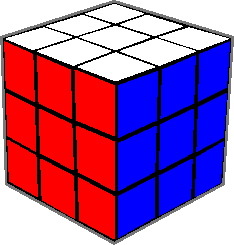
\includegraphics[width=60pt]{figs/hungarian_cube.pdf}
\end{column}
\begin{column}{0.5\textwidth}
A \alert{Hasse diagram} of a simplicial complex (vertices named for the colors on a Hungarian Cube)
\end{column}
\end{columns}
\end{frame}

\begin{frame}{Higher realization}
\begin{columns}
\begin{column}{0.5\textwidth}
\begin{tikzpicture}
  \draw
    (0, 0) grid[step=1cm] (3, 3)
    (0, 2) edge[ultra thick] (1, 3)
    (0, 1) edge[ultra thick] (0, 2)
    (0, 1) edge[ultra thick] (1, 1)
    (1, 1) edge[ultra thick] (2, 2)
    (2, 2) edge[ultra thick] (2, 3)
    (1, 3) edge[ultra thick] (2, 3)
    (0, 1) -- (2, 3)
    (0, 0) -- (3, 3)
    (1, 0) -- (3, 2)
    (2, 0) -- (3, 1);
  \fill[radius=3pt]
    \foreach \x in {0, ..., 3} {
      \foreach \y in {0, ..., 3} {
        (\x, \y) circle[]
    }};
  \path[above left]
    \foreach \p/\v in {
      {1, 3}/a,
      {2, 3}/b,
      {0, 2}/f,
      {1, 2}/v,
      {2, 2}/c,
      {0, 1}/e,
      {1, 1}/d%
    } {
      (\p) node {$\v$}
    };
\end{tikzpicture}

\end{column}
\begin{column}{0.5\textwidth}
The \defemph{link} of a vertex \( v \) in an \( n \)-complex is the \( (n-1) \)-subcomplex of faces not containing \( v \) but whose union with \( v \) is a face.\\~\\

This will be our model of the tangent space.
\end{column}
\end{columns}
\end{frame}

\begin{frame}[c]{Higher realization}
\begin{columns}[T]
\begin{column}{0.4\textwidth}
\begin{minipage}[t][0.7\textheight]{\textwidth}
% https://q.uiver.app/#q=WzAsNCxbMCwxLCJNXzA9XFxtYXRoYmJ7TX1fMCJdLFsxLDEsIlxcbWF0aGJie019XzEiXSxbMSwwLCJNXzEiXSxbMCwwLCJNXzFcXHRpbWVzIFxcYmRzaW1wbGV4bnsxfSJdLFswLDFdLFszLDAsIlxcbWF0aGJie0F9XzAiLDJdLFszLDIsIlxcbWF0aHJte3ByfV8xIl0sWzIsMSwiKl97XFxtYXRoYmJ7TX1fMX0iXSxbMSwzLCIiLDIseyJvZmZzZXQiOjMsInN0eWxlIjp7Im5hbWUiOiJjb3JuZXItaW52ZXJzZSJ9fV0sWzAsMiwiaF8xIiwyLHsic2hvcnRlbiI6eyJzb3VyY2UiOjQwLCJ0YXJnZXQiOjQwfSwibGV2ZWwiOjJ9XV0=
\begin{tikzcd}
  {M_1\times \bdsimplexn{1}} & {M_1} \\
  {M_0=\mathbb{M}_0} & {\mathbb{M}_1}
  \arrow["{\mathrm{pr}_1}", from=1-1, to=1-2]
  \arrow["{\mathbb{A}_0}"', from=1-1, to=2-1]
  \arrow["{*_{\mathbb{M}_1}}", from=1-2, to=2-2]
  \arrow["{h_1}"', shorten <=14pt, shorten >=14pt, Rightarrow, from=2-1, to=1-2]
  \arrow[from=2-1, to=2-2]
  \arrow["\ulcorner"{pos=0, rotate=180}, shift left=1, draw=none, from=2-2, to=1-1]
\end{tikzcd}


\vspace{\fill}
Form a pushout of edges to create a 1-type.
\end{minipage}
\end{column}
\begin{column}{0.6\textwidth}
\begin{minipage}[t][0.7\textheight]{\textwidth}
% https://q.uiver.app/#q=WzAsNyxbMCwyLCJNXzFcXHRpbWVzIFxcYmRzaW1wbGV4bnsxfSJdLFswLDEsIlxcbWF0aGJie019XzAiXSxbMSwxLCJcXG1hdGhiYntNfV8xIl0sWzEsMiwiTV8xIl0sWzEsMCwiTV8yXFx0aW1lcyBcXGJkc2ltcGxleG57Mn0iXSxbMiwwLCJNXzIiXSxbMiwxLCJcXG1hdGhiYntNfV8yIl0sWzAsMSwiXFxtYXRoYmJ7QX1fMCJdLFsxLDJdLFswLDMsIlxcbWF0aHJte3ByfV8xIiwyXSxbMywyLCIqX3tcXG1hdGhiYntNfV8xfSIsMl0sWzIsMCwiIiwxLHsic3R5bGUiOnsibmFtZSI6ImNvcm5lci1pbnZlcnNlIn19XSxbMiw2XSxbNCwyLCJcXG1hdGhiYntBfV8xIiwyXSxbNSw2LCIqX3tcXG1hdGhiYntNfV8yfSJdLFs0LDUsIlxcbWF0aHJte3ByfV8xIl0sWzYsNCwiIiwxLHsic3R5bGUiOnsibmFtZSI6ImNvcm5lci1pbnZlcnNlIn19XSxbMiw1LCJoXzIiLDAseyJzaG9ydGVuIjp7InNvdXJjZSI6NDAsInRhcmdldCI6NDB9LCJsZXZlbCI6Mn1dLFsxLDMsImhfMSIsMix7InNob3J0ZW4iOnsic291cmNlIjo0MCwidGFyZ2V0Ijo0MH0sImxldmVsIjoyfV1d
\begin{tikzcd}
  & {M_2\times \bdsimplexn{2}} & {M_2} \\
  {\mathbb{M}_0} & {\mathbb{M}_1} & {\mathbb{M}_2} \\
  {M_1\times \bdsimplexn{1}} & {M_1}
  \arrow["{\mathrm{pr}_1}", from=1-2, to=1-3]
  \arrow["{\mathbb{A}_1}"', from=1-2, to=2-2]
  \arrow["{*_{\mathbb{M}_2}}", from=1-3, to=2-3]
  \arrow[from=2-1, to=2-2]
  \arrow["{h_1}"', shorten <=27pt, shorten >=27pt, Rightarrow, from=2-1, to=3-2]
  \arrow["{h_2}", shorten <=17pt, shorten >=17pt, Rightarrow, from=2-2, to=1-3]
  \arrow[from=2-2, to=2-3]
  \arrow["\ulcorner"{anchor=center, pos=0.125, rotate=-135}, draw=none, from=2-2, to=3-1]
  \arrow["\ulcorner"{anchor=center, pos=0.125, rotate=180}, draw=none, from=2-3, to=1-2]
  \arrow["{\mathbb{A}_0}", from=3-1, to=2-1]
  \arrow["{\mathrm{pr}_1}"', from=3-1, to=3-2]
  \arrow["{*_{\mathbb{M}_1}}"', from=3-2, to=2-2]
\end{tikzcd}


\vspace{\fill}
Then push out maps from a 1-type triangle to from a 2-dim type.
\end{minipage}
\end{column}
\end{columns}
\end{frame}

\begin{frame}{Higher realization}
% https://q.uiver.app/#q=WzAsNyxbMCwyLCJNXzFcXHRpbWVzIFxcYmRzaW1wbGV4bnsxfSJdLFswLDEsIlxcbWF0aGJie019XzAiXSxbMSwxLCJcXG1hdGhiYntNfV8xIl0sWzEsMiwiTV8xIl0sWzEsMCwiTV8yXFx0aW1lcyBcXGJkc2ltcGxleG57Mn0iXSxbMiwwLCJNXzIiXSxbMiwxLCJcXG1hdGhiYntNfV8yIl0sWzAsMSwiXFxtYXRoYmJ7QX1fMCJdLFsxLDJdLFswLDMsIlxcbWF0aHJte3ByfV8xIiwyXSxbMywyLCIqX3tcXG1hdGhiYntNfV8xfSIsMl0sWzIsMCwiIiwxLHsic3R5bGUiOnsibmFtZSI6ImNvcm5lci1pbnZlcnNlIn19XSxbMiw2XSxbNCwyLCJcXG1hdGhiYntBfV8xIiwyXSxbNSw2LCIqX3tcXG1hdGhiYntNfV8yfSJdLFs0LDUsIlxcbWF0aHJte3ByfV8xIl0sWzYsNCwiIiwxLHsic3R5bGUiOnsibmFtZSI6ImNvcm5lci1pbnZlcnNlIn19XSxbMiw1LCJoXzIiLDAseyJzaG9ydGVuIjp7InNvdXJjZSI6NDAsInRhcmdldCI6NDB9LCJsZXZlbCI6Mn1dLFsxLDMsImhfMSIsMix7InNob3J0ZW4iOnsic291cmNlIjo0MCwidGFyZ2V0Ijo0MH0sImxldmVsIjoyfV1d
\begin{tikzcd}
  & {M_2\times \bdsimplexn{2}} & {M_2} \\
  {\mathbb{M}_0} & {\mathbb{M}_1} & {\mathbb{M}_2} \\
  {M_1\times \bdsimplexn{1}} & {M_1}
  \arrow["{\mathrm{pr}_1}", from=1-2, to=1-3]
  \arrow["{\mathbb{A}_1}"', from=1-2, to=2-2]
  \arrow["{*_{\mathbb{M}_2}}", from=1-3, to=2-3]
  \arrow[from=2-1, to=2-2]
  \arrow["{h_1}"', shorten <=27pt, shorten >=27pt, Rightarrow, from=2-1, to=3-2]
  \arrow["{h_2}", shorten <=17pt, shorten >=17pt, Rightarrow, from=2-2, to=1-3]
  \arrow[from=2-2, to=2-3]
  \arrow["\ulcorner"{anchor=center, pos=0.125, rotate=-135}, draw=none, from=2-2, to=3-1]
  \arrow["\ulcorner"{anchor=center, pos=0.125, rotate=180}, draw=none, from=2-3, to=1-2]
  \arrow["{\mathbb{A}_0}", from=3-1, to=2-1]
  \arrow["{\mathrm{pr}_1}"', from=3-1, to=3-2]
  \arrow["{*_{\mathbb{M}_1}}"', from=3-2, to=2-2]
\end{tikzcd}


\( *_{\mm_1}, *_{\mm_2} \) provide \alert{hubs}.

\( h_1, h_2 \) provide \alert{spokes}.
\end{frame}

\begin{frame}
\begin{definition}
An \defemph{\( n \)-gon} \( \ccc(n) \) is the realization of a complex \( C(n) \):
\vspace{-10pt}\begin{align*}
C(n)_0 &= \{v_1,\ldots,v_n\} \\
C(n)_1 &= \{e_1=\{v_1,v_2\}, \ldots, e_{n-1}=\{v_{n-1}, v_n\}, e_n=\{v_n, v_0\}\}
\end{align*}
\end{definition}
\vspace{-10pt}Toss in the non-complexes \vspace{-20pt}
\[ \ccc(1)\defeq S^1,\quad \ccc(2)\defeq \begin{tikzpicture}[scale=0.5, baseline=3.5mm]
\tikzset{arrow/.style={-{Stealth[scale=1.1]}}}
\tikzset{oo/.style={circle, scale=0.25, fill=black}}
\tikzset{ooo/.style={circle, scale=0.25, fill=none}}
\node[oo, label=above:\( v_1 \)] (V1) at (0, 2) {};
\node[oo, label=below:\( v_2 \)] (V2) at (0, 0) {};
\node[ooo] (V21) at (0.3, 1.75) {};
\node[ooo] (V22) at (0.3, 0.25) {};
\draw (V1) edge[bend right=60, swap, "\( \ell_{12} \)"] (V2);
\draw (V1) edge[bend left=60, "\( r_{21} \)"] (V2);
\end{tikzpicture}\]
We sometimes denote a polygon with vertices \( \{a, b, c\} \) with \( \gr{abc} \), its realization with \( \hgr{abc} \).
\end{frame}

\begin{frame}
\begin{lemma}
\( \ccc(2)\simeq \ccc(1) \) and in general \( \ccc(n)\simeq\ccc(n-1) \).
\end{lemma}
\begin{corollary}
All \( n \)-gons are equivalent to \( S^1 \) and so provide terms in \( \EMzo \).
\end{corollary}
\end{frame}

\begin{frame}{Rotation}
Let \( R:\gr{abcd}\to\gr{abcd} \) send \( a\mapsto b , b\mapsto c , c\mapsto d, d\mapsto a \). \\~\\

Extend \( R \) to edges.

\begin{lemma}
\( \hgr{R}:\hgr{abcd}\to\hgr{abcd} \) is homotopic to the identity, i.e. we have \( \pit{x:\hgr{abcd}}x=\hgr{R}(x) \).
\end{lemma}
\begin{proof}
Use edges.
\end{proof}
\end{frame}

\section{Connections and curvature}
\begin{frame}
\begin{definition}
If \( \mm\defeq \mm_0\xrightarrow[]{\imath_0}\cdots\xrightarrow[]{\imath_{n-1}}\mm_n \) is a cellular type and all the triangles commute in the diagram:\vspace{-10pt}
\[\begin{tikzcd}[ampersand replacement=\&, column sep=small]
  {\mm_0} \& {\mm_1} \& {\mm_2} \& \cdots \& {\mm_n} \\
\&\& {\mathcal{U}}
\arrow["{\imath_0}", from=1-1, to=1-2]
\arrow["{f_0}", from=1-1, to=2-3]
\arrow["{\imath_1}", from=1-2, to=1-3]
\arrow["{f_1}", from=1-2, to=2-3]
\arrow["{\imath_2}", from=1-3, to=1-4]
\arrow["{f_2}", from=1-3, to=2-3]
\arrow["{\imath_{n-1}}", from=1-4, to=1-5]
\arrow["f_n"', from=1-5, to=2-3]
\end{tikzcd}\]\vspace{-15pt}
\begin{itemize}
\item The map \( f_k \) is a \defemph{\( k \)-bundle} on \( \mm \).
\item The pair given by the map \( f_k \) and the proof \( f_k\circ \imath_{k-1}=f_{k-1} \), i.e. that \( f_k \) extends \( f_{k-1} \) is called a \defemph{\( k \)-connection on the \( (k-1) \)-bundle \( f_{k-1} \)}.
\end{itemize}
\end{definition}
\end{frame}

\begin{frame}
\begin{mydef}
If \( \mm \) is the realization of a simplicial complex and we have 
\begin{center}
\begin{tikzcd}[ampersand replacement=\&, column sep=small, row sep=small]
  {M_k\times \partial\Delta^k} \& {M_k} \\
  {\mathbb{M}_{k-1}} \& {\mathbb{M}_k} \\
  \& {\mathcal{U}}
  \arrow["{\mathrm{pr}_1}", from=1-1, to=1-2]
  \arrow["{\mathbb{A}_{k-1}}"', from=1-1, to=2-1]
  \arrow["{*_{\mathbb{M}_k}}", from=1-2, to=2-2]
  \arrow["{h_k}", shorten <=10pt, shorten >=10pt, Rightarrow, from=2-1, to=1-2]
  \arrow["{\imath_{k-1}}", from=2-1, to=2-2]
  \arrow[""{name=0, anchor=center, inner sep=0}, "{f_{k-1}}"', from=2-1, to=3-2]
  \arrow["\ulcorner"{anchor=center, pos=0.125, rotate=180}, draw=none, from=2-2, to=1-1]
  \arrow["{f_k}", from=2-2, to=3-2]
  \arrow[shorten >=3pt, Rightarrow, from=2-2, to=0]
\end{tikzcd}
\begin{tikzcd}[ampersand replacement=\&]
  {\{m_k\}\times \partial\Delta^k} \& \unit \\
  {\mathbb{M}_{k-1}} \& {\mathcal{U}}
  \arrow["{!}", from=1-1, to=1-2]
  \arrow["{\mathbb{A}_{k-1}}"', from=1-1, to=2-1]
  \arrow["{*_{\mathbb{M}_k}}", from=1-2, to=2-2]
  \arrow["{\flat_k}", shorten <=11pt, shorten >=11pt, Rightarrow, from=1-2, to=2-1]
  \arrow[from=2-1, to=2-2]
\end{tikzcd}
\end{center}
then we say the filler \( \flat_k \) is called a \defemph{flatness structure for the face \( m_k \)}, and its ending path is called \defemph{curvature at the face \( m_k \)}.
\end{mydef}
\end{frame}

\section{Results}

\begin{frame}{Classical proof}
\begin{columns}
\column{0.5\textwidth}
\begin{figure}
\includegraphics[width=0.9\textwidth]{figs/needham_triangle.pdf}
\caption{from Tristan Needham, \emph{Visual Differential Geometry and Forms}}
\end{figure}
\column{0.5\textwidth}
\begin{itemize}
\item The classical proof is discrete-flavored.
\item ``\( \angle Fw_{||} \)'' looked a lot like a pathover.
\item Hopf's \( \Phi \) is defined on edges, not loops. We imitated that too.
\end{itemize}
\end{columns}
\end{frame}




\end{document}
